\subsection{Sistema Bevim}

O sistema BeVim é composto pelos seguintes módulos:

\begin{itemize}
	\item Módulo de Sensoriamento - Parte responsável pela leitura de sensores, comunicação com a CPU e controle dos módulos de motores. 
	\item Módulo de Motor - Parte responsável pelo controle de inversores, e pela retroalimentação em malha fechada para atingir frequencias altas.
\end{itemize}

Ambos os moódulos são conectados entre si por uma rede I2C (InterIntegrated Circuits), onde o módulo de sensoriamento sempre atua como mestre no processo de comunicação. Esse procedimento foi escolhido pela possibilidade de se adicionar de maneira fácil outros módulos (de motor, por exemplo, ou outros que sejam de interesse a serem desenvolvidos), não interferindo com outros sistemas perifericos a mesa.

\subsubsection{Módulo de Sensoriamento}
O módulo de sensoriamento é o responsável pela implementação da interface (via protocolo BeVim) com o sistema que controla a mesa em alto nível - a CPU. Ao mesmo tempo, esse módulo executa um controle da leitura dos sensores digitais do projeto, e dos outros módulos acoplados (os de motores).

\begin{figure}[htbp]
	\centering
		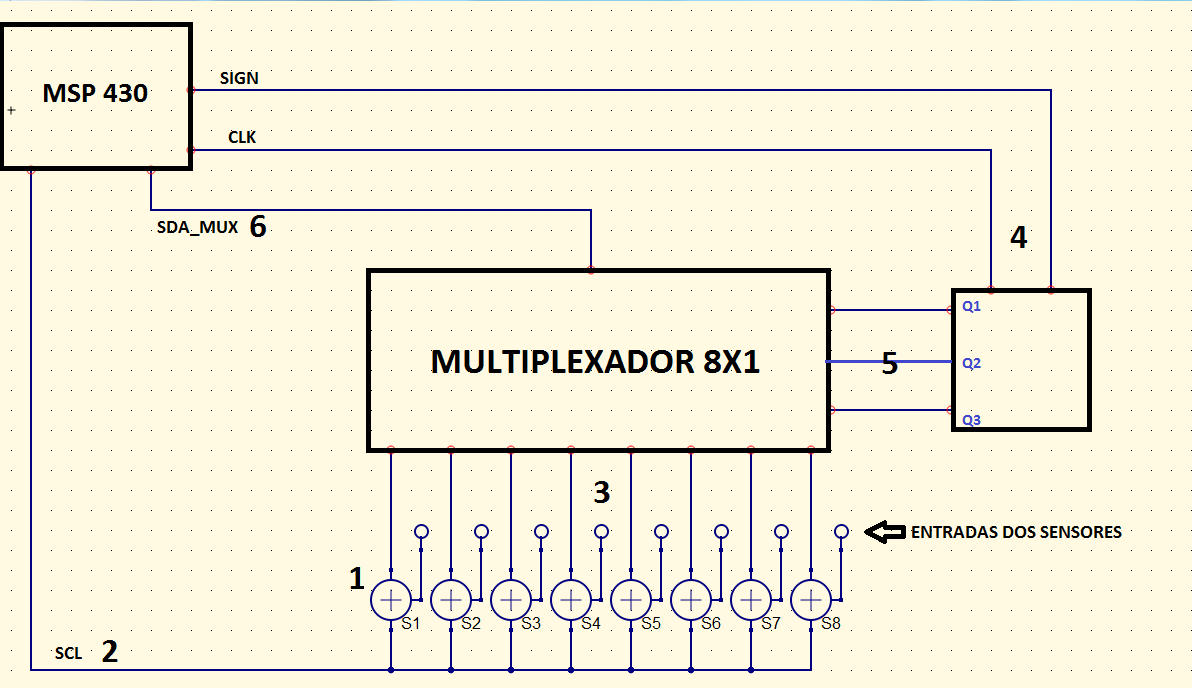
\includegraphics[scale=0.6]{mod_sensor.png}
	\caption{Módulo de Sensoriamento}
	\label{mod_sensor}
\end{figure}

Itens da Figura \ref{mod_sensor}:

\begin{enumerate}
	\item Conectores DB9, que receptam os sinais dos acelerômetros.
	\item Os sensores recebem sinais de clock provindos do microcontrolador, através do sinal “SCL” da rede I2C.
	\item Os sinais de dados de cada sensor servem como entrada de um multiplexador 8x1.
	\item O MSP430, através de duas portas GPIO's, controlam um registrador responsável pelas portas seletoras do multiplexador. Uma porta é o sinal serial de seleção “sign” e a outra é o clock “clk”.
	\item O conjunto do registrador com o multiplexador é capaz de selecionar qual sensor será aferido pelo sistema.
	\item O dado do sensor selecionado é enviado para a rede I2C através do caminho “SDA_MUX”
\end{enumerate}

\subsubsection{Módulo de Motor}

\begin{figure}[htbp]
	\centering
		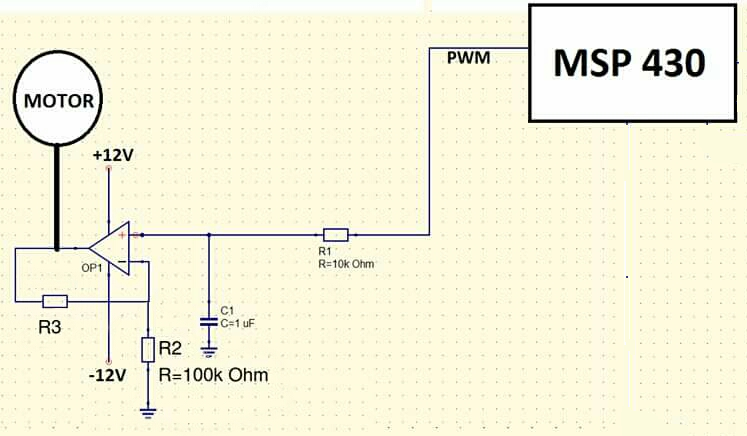
\includegraphics[scale=0.6]{mod_motor.png}
	\caption{Módulo do Motor}
	\label{mod_motor}
\end{figure}

 
\subsection{Circuito Completo}

\begin{figure}[htbp]
	\centering
		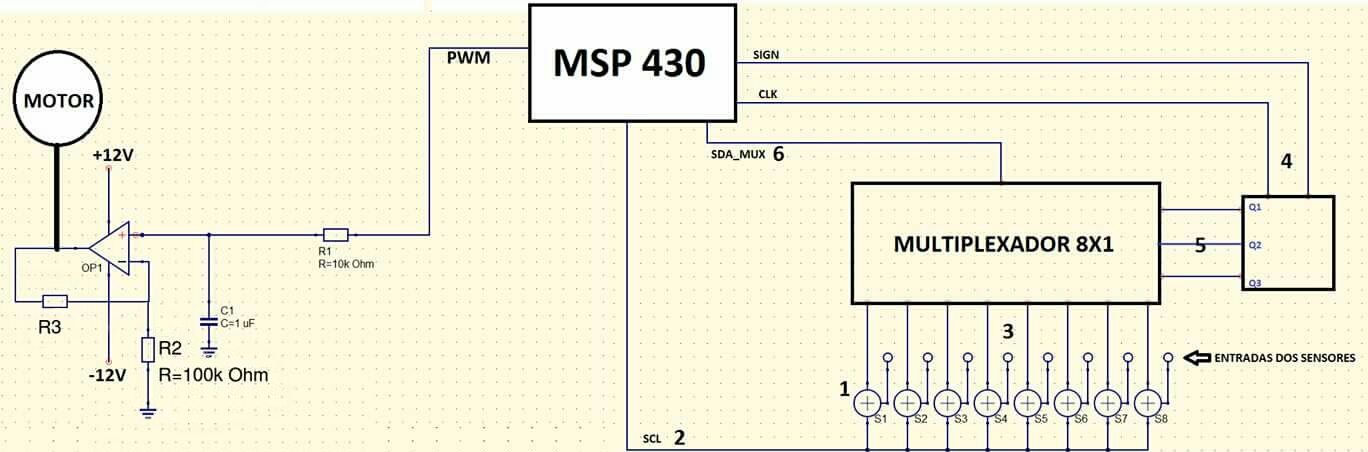
\includegraphics[scale=0.6]{mod_completo.png}
	\caption{Circuito Completo}
	\label{mod_completo}
\end{figure}
